\newcommand\SLASH{\char`\\}

\section{Protocol Design}

\subsection{Protocol Overview}

\begin{figure}[!h]
    \begin{center}
        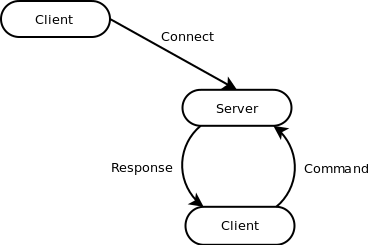
\includegraphics[scale=0.65]{chapter2/diagrams/protocol_high_level.png}
        \caption{The exchange of messages between a client and the server}
        \label{highLevelDia}
    \end{center}
\end{figure}

Gim uses a client-server architecture, where one computer (known as the Sever) acts as a central point to which other computers (the Clients) connect. The clients do not communicate directly with each other and all communication takes place between the clients and the server. If a client wishes to send a message to another client it must first got through the server.

In GIM, the Protocol is responsible for enabling communication between the clients and the server in a reliable and consistent manner. A protocol is a set of rules that determine the format and transmission of data between computers. The syntax (the structure, or format) and semantics (the meaning) of the Protocol are discussed in the next section.

At the highest level of abstraction, the GIM Protocol works in a very simple manner.  A client connects to the sever and they exchange messages until the connection is closed, as shown in Figure ~\ref{highLevelDia}.

In practice there are several clients connected to the server at once, however as the clients do not directly interact with each other and do not need to know about each other, the entire system can be described as above.

\subsection{Protocol Specification}
\subsubsection{Syntax}

The GIM Protocol uses a simple, text based syntax. Each full command begins with a colon followed by a command name and its arguments. A second colon marks the end of the headers and beginning of the data segment. A semi-colon marks the end of the data segment and the termination of the command. The basic structure of a full command is shown below:

\texttt{:<COMMAND\_NAME> <ARGUMENTS>: <DATA>;}

Commands names are predefined and \texttt{<COMMAND\_NAME>} can be any 1 of the following 19 values:

\texttt{
\begin{tabular}{ | p{3.3cm} |p{3.3cm}  |p{3.3cm} |p{3.3cm} | } 
    \hline
    AUTH & FRIENDREQUEST & MESSAGE & ROOM \\
    \hline
    BROADCAST & GET & OKAY & SERVERSTATUS \\
    \hline
    ERROR & INFO &PING & SET \\
    \hline
    FRIEND & KILL & PONG & UPDATE \\
    \hline
    FRIENDLIST & LOGOUT & QUIT & \\
    \hline
 \end{tabular}
 }
 
\texttt{<ARGUMENTS>} is a set of 0 or more predefined arguments which can be passed to the command in order to change its behaviour. Each command has its own set of arguments, some commands require arguments, some commands accept more than one argument and some commands have no arguments. The protocol specification defines over 60 arguments and a full listing for each command can be found in the \emph{GIM Protocol Specification Document}.

Unlike the command and arguments segments, the \texttt{<DATA>} segment does not have predefined values and has a varying syntax across different commands. The majority of the data is likely to have been provided by the user at some point, and as such the data segment is considered to be ``unsafe" and is encoded (See \emph{Encoding, Limits and Restrictions} for information about how the data is encoded). A full specification for the data segment of each command can be found in the \emph{GIM Protocol Specification Document}.

For example, the following is an example of a command sent from the client to the server requesting the Nickname and Status of the users joe@example.com and bill@gmail.org:

\texttt{:GET NICKNAME STATUS: joe\SLASH U+0040example.com bill\SLASH U+0040mail.org;}

To which the server may reply:

\texttt{:INFO NICKNAME STATUS: joe\SLASH U+0040example.com\\
Jeo\\
ONLINE\\
bill\SLASH U+0040mail.org\\
Billy The Kid\\
AWAY;}

\emph{(Please note that the data segments is the previous examples have been encoded as is defined below in Encoding, Limits and Restrictions.)}

\subsubsection{Roles and States}
The protocol defines two separate roles: The Client role and the Server role. Each role is only able to send a specific subset of commands but must also be able to receive and understand all of the commands sent by the opposite role. This means that both the client and server must implement all of the commands in some way.

Having clearly defined roles is an integral part of the GIM Protocol. This allows the semantics of a command to be used to generate a response in cases where both roles are able to send and receive a command but where the command has a different meaning depending on its source. 

For example, the \texttt{AUTH} command can be sent by both the client and the server roles. When sent by the server it is used to indicate the current state of the client (Either Logged-in or Unauthorized) but when sent by the client it indicates that they wish to login or register a new account. This means that the same command must be implemented differently depending on the role of the sender.

As mentioned above, the client role has 2 states: Logged-in and Unauthorized. When the client first establishes a connection it is placed in the unauthorized state. This means that it has access to an even smaller subset of commands, only those essential to logging-in or registering a new account. Once the client has successfully logged-in it is granted access to the full set of client commands.

\subsubsection{Security and Encryption}

\subsubsection{Encoding, Limits and Restrictions}

\subsection{Protocol Evolution}
